\chapter{Funzionalità e relative implementazioni}
\section{Gestione utenze}
Le utenze in Garzone sono rappresentate da singoli record sulla base di dati a cui sono referenziate istanze di utenze su vari servizi esterni. Ogni utenza della piattaforma ha in particolare associato un record su:
\begin{itemize}
    \item \textbf{Firebase Authentication}: per la parte vera e propria di registrazione, autenticazione e gestione delle sessioni
    \item \textbf{CloudSQL}: dove vengono memorizzati i dettagli principali relativi all'utenza
    \item \textbf{Mailchimp}: dove viene creata un'utenza utile ai fini di marketing e engagement
    \item \textbf{Stripe}: dove viene creata un'utenza a cui vengono collegati i vari pagamenti effettuati/ricevuti e i dettagli di fatturazione
\end{itemize}
Ad ogni utenza viene assegnato il ruolo a cui appartiene, per poi consentire l'accesso alla singola piattaforma dedicata, ad esempio un negozio può autenticarsi solamente sul pannello a lui dedicato, così come amministratori, utenti e comuni. Questa funzionalità è messa a disposizione da Firebase Authentication attraverso l'utilizzo dei \textit{custom claims}, ovvero un oggetto che al suo interno contiene dati di tipo chiave-valore assegnati in fase di registrazione e utilizzati per distinguere i vari tipi di utenza.
\begin{figure}[h!]
    \centering
    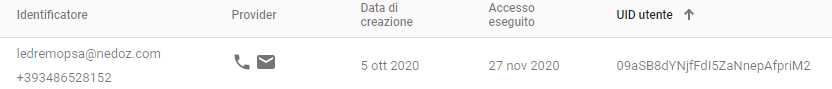
\includegraphics[width=1\textwidth]{recordfb.png}
    \caption{Record utenza Garzone su Firebase Authentication}
\end{figure}
\FloatBarrier
Dal pannello di amministrazione è possibile abilitare/disabilitare l'accesso alle varie piattaforme per ogni utente registrato. Questa operazione avviene cambiando il valore del flag \textit{<<abilitato>>} presente in ogni istanza di utenza sulla base di dati e controllando ad ogni cambio di route l'effettiva abilitazione. Ogni richiesta effettuata dal client alla componente backend viene recepita e accettata solo nel caso in cui la sorgente disponga delle autorizzazioni necessarie, altrimenti è compito della singola function restituire una risposta provvista di errore.
\subsection{Registrazione}
La procedura di registrazione prevede, per i pannelli di negozi e utenti, una fase di landing su una precisa pagina dell'applicativo accessibile da tutti i client che ne fanno richiesta. Dopo la compilazione dei campi e la loro validazione è compito della componente di backend eseguire le seguenti operazioni:
\begin{enumerate}
    \item Destrutturare i parametri della richiesta 
    \item Ri-validare i parametri della richiesta
    \item Interfacciarsi al servizio di Firebase Authentication per la creazione dell'utenza
    \item Invio della mail di verifica dell'account
    \item Interfacciarsi eventualmente al servizio di geolocalizzazione per il computo delle coordinate geografiche dato l'indirizzo in un parametro della richiesta
    \item Generare l'istanza dell'utenza provvista dei dettagli forniti nei parametri della richiesta e inserirla nel database relazionale 
    \item Assegnare i custom claims all'utenza generata su Firebase
    \item Interfacciarsi al servizio esterno Mailchimp per la creazione dell'utenza associata
    \item Restituire alla componente frontend il risultato dell'operazione
\end{enumerate}
\begin{figure}[h!]
    \centering
    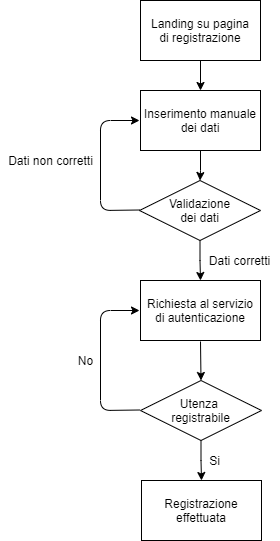
\includegraphics[width=0.4\textwidth]{registrazione.png}
    \caption{Flusso di registrazione di un negozio}
\end{figure}
\FloatBarrier
La procedura di registrazione, per questioni di sicurezza non è prevista per comuni e amministratori. Questa operazione per l'amministratore superuser è stata prevista inizialmente, mentre per i comuni viene eseguita dal pannello di amministrazione.
\newpage
\subsection{Accesso}
La fase di accesso, presente su ogni pannello, prevede l'inserimento delle credenziali di accesso fornite dall'utente in fase di registrazione. Il servizio backend fornito da Firebase Authentication provvede poi a verificarle e a fornire una risposta al client che ha richiesto l'accesso. Per ottenere l'accesso alla piattaforma sono necessari tre requisiti:
\begin{itemize}
    \item Registrazione effettuata con successo
    \item Custom claim relativo al ruolo dell'utenza corrispondente al pannello dove si vuole effettuare la procedura di accesso
    \item Email già verificata in precedenza
    \item Account abilitato su firebase
    \item Account abilitato sulla base di dati
\end{itemize}

\begin{figure}[h!]
    \centering
    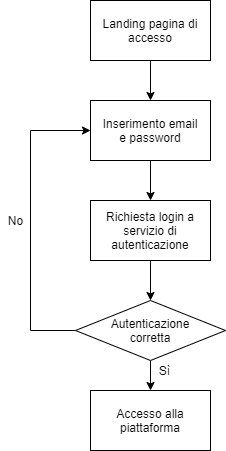
\includegraphics[width=0.4\textwidth]{login.png}
    \caption{Flusso di login del negozio}
\end{figure}
\FloatBarrier
Per una corretta gestione dei claims è presente, in tutti gli applicativi frontend, un listener (procedura che in runtime resta in ascolto di un endpoint del backend) che ha il compito di verificare a intervalli costanti i permessi dell'utenza e, nel caso non fossero coerenti, di effettuare la procedura di logout.
\paragraph{Private Route} Nell'applicativo, ad ogni navigazione verso pagine diverse dalla corrente, è previsto, per le route private, una serie di controlli per evitare che un utente non autorizzato acceda a sezioni di Garzone a lui non consentite. Questa funzionalità è prevista dal componente \lstinline[basicstyle=\ttfamily]!PrivateRoute!, che renderizza il componente \lstinline[basicstyle=\ttfamily]!Route! (lo screen richiesto), solo dopo aver effettuato tutti i con trolli necessari.
\begin{figure}[h!]
    \centering
    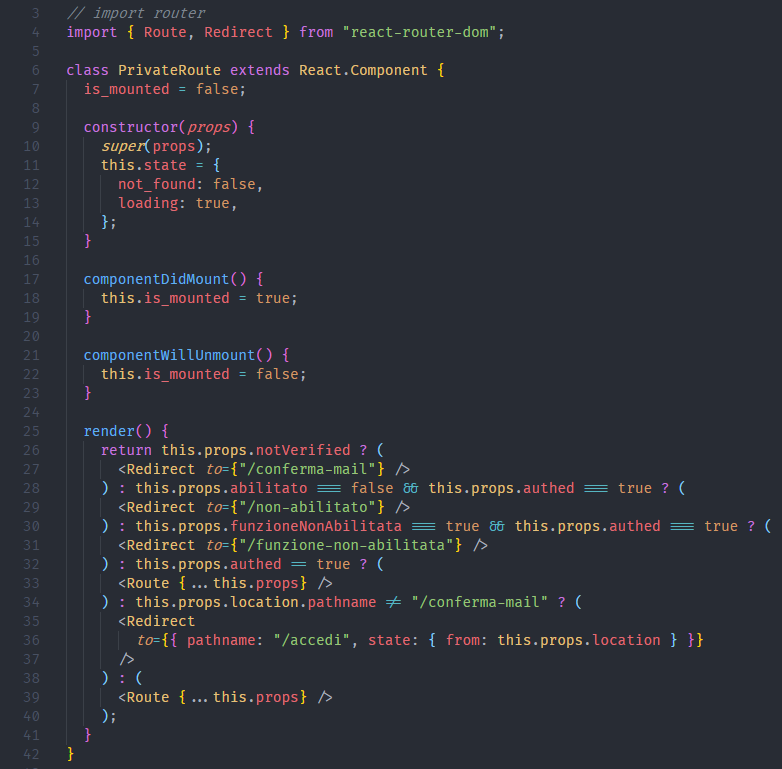
\includegraphics[width=1\textwidth]{private.png}
    \caption{Componente \lstinline[basicstyle=\ttfamily]!PrivateRoute!}
\end{figure}
\FloatBarrier
\section{Catalogo Prodotti e Catalogo Servizi}
Ogni negoziante ha la possibilità, tramite il proprio pannello, di inserire e gestire sia prodotti che servizi del suo catalogo. Successivamente i record generati possono essere visionati dagli utenti dall'apposita piattaforma e gestiti inoltre dall'amministrazione.
\paragraph{Entità} Un prodotto o un servizio da registrare necessita di dati relativi a nome, descrizione, categoria, immagine, prezzo, prezzo scontato e flag di messa in vendita.
\begin{figure}[h!]
    \begin{subfigure}{0.5\textwidth}
    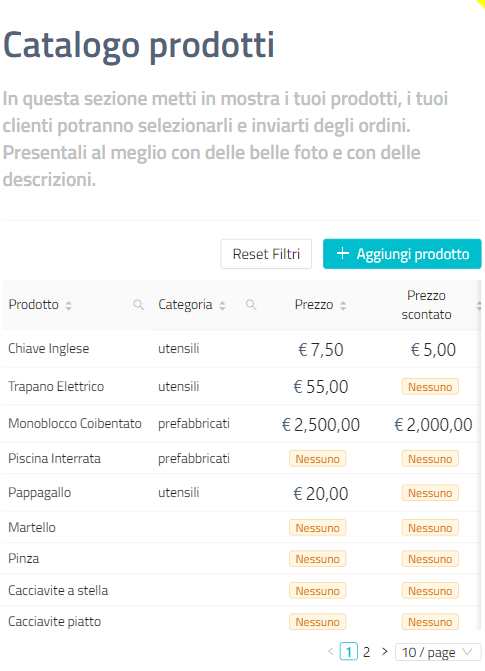
\includegraphics[width=0.9\linewidth]{pannellopr.png} 
    \caption{Gestione prodotti - Pannello negozio}
    \label{fig:subim1}
    \end{subfigure}
    \begin{subfigure}{0.5\textwidth}
    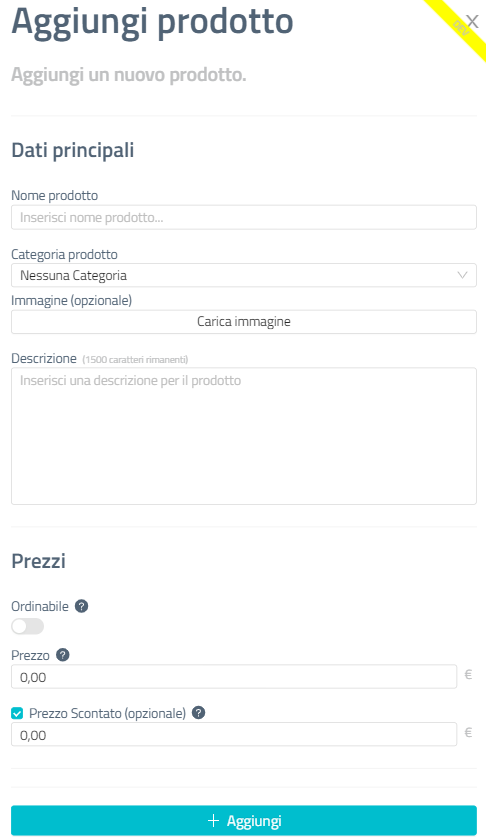
\includegraphics[width=0.9\linewidth]{drawerpr.png}
    \caption{Aggiunta prodotto - Pannello negozio}
    \label{fig:subim2}
    \end{subfigure}
    
    \caption{Schermate di Garzone relaitive al catalogo prodotti}
    \label{fig:image2}
\end{figure}
\FloatBarrier
Dal pannello di gestione è inoltre prevista la funzionalità di ricerca e filtraggio dei dati in base a parametri scelti dall'utente. Per la fase di registrazione di prodotti e servizi, data la necessità di allegare immagini, è previsto l'utilizzo del bucket di Firebase. In caso di cancellazione del record è necessaria quindi l'eliminazione del file associato all'immagine dal bucket stesso.
\section{Promozioni}
Altra funzionalità fornita ai negozi è relativa alla creazione e gestione di promozioni, ovvero annunci visionabili dagli utenti provvisti di data di scadenza. Per la gestione delle date è stata utilizzata la libreria \lstinline[basicstyle=\ttfamily]!moment.js!, che fornisce semplificazioni riguardo le operazioni da eseguire sulla validazione dei dati in fase di creazione e di modifica.
\paragraph{Entità} Una promozione necessita di dati relativi a titolo, descrizione, data di scadenza e un immagine esplicativa.
\begin{figure}[h!]
    \begin{subfigure}{0.5\textwidth}
    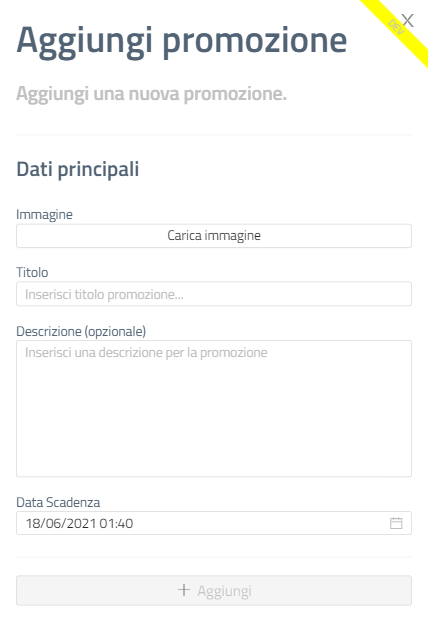
\includegraphics[width=0.9\linewidth]{drawerpro.png} 
    \caption{Aggiunta promozione - Pannello negozio}
    \label{fig:subim1}
    \end{subfigure}
    \begin{subfigure}{0.5\textwidth}
    
\includegraphics[width=0.9\linewidth]{espro.png}
    \caption{Promozione - Garzone}
    \label{fig:subim2}
    \end{subfigure}
    
    \caption{Schermate di Garzone relative alle promozioni}
    \label{fig:image2}
\end{figure}
\section{Ordini}
Una delle funzionalità più rilevanti all'interno di Garzone è sicuramente quella relativa alla creazione e alla gestione degli ordini. Un ordine viene generato da un utente da un'iniziale composizone di un carrello con prodotti selezionati dalla navigazione tra i cataloghi di un negozio. Dopo aver composto il carrello è possibile per l'utente procedere con la creazione dell'ordine, inserendo dati relativi a modalità di consegna, modalità di pagamento, eventuali note per il negozio ed eventuale indirizzo di consegna. Sarà poi compito del negozio confermare l'ordine ricevuto e procedere con la sua evasione, richiedendo eventualmente il pagamento online per gli ordini che lo prevedono. 
\begin{figure}[h!]
    \centering
    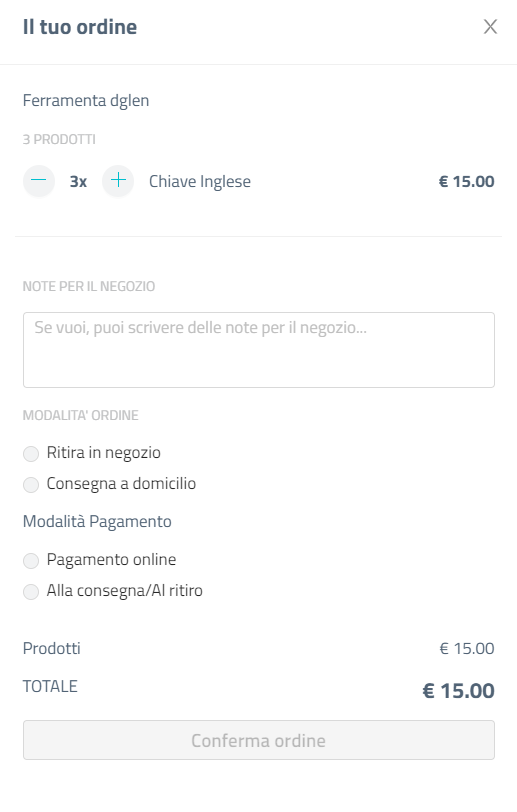
\includegraphics[width=0.5\textwidth]{ordine.png}
    \caption{Form di creazione ordine}
\end{figure}
Il negozio ha il compito infine di gestire l'avanzamento di stato dell'ordine dal proprio pannello di controllo, terminandone l'evasione selezionando il relativo status "consegnato". Ad ogni passaggio di status dell'ordine, la componente di backend ha il compito di notificare correttamente sia l'utente sia il negozio coinvolti tramite notifiche push e email transazionali. 
\begin{figure}[h!]
    \begin{subfigure}{0.5\textwidth}
    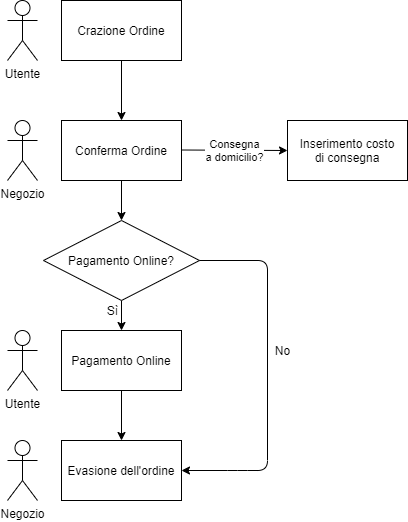
\includegraphics[width=1\linewidth]{flussoord.png}
    \caption{Flusso di gestione di un ordine}
    \label{fig:subim1}
    \end{subfigure}
    \begin{subfigure}{0.5\textwidth}
    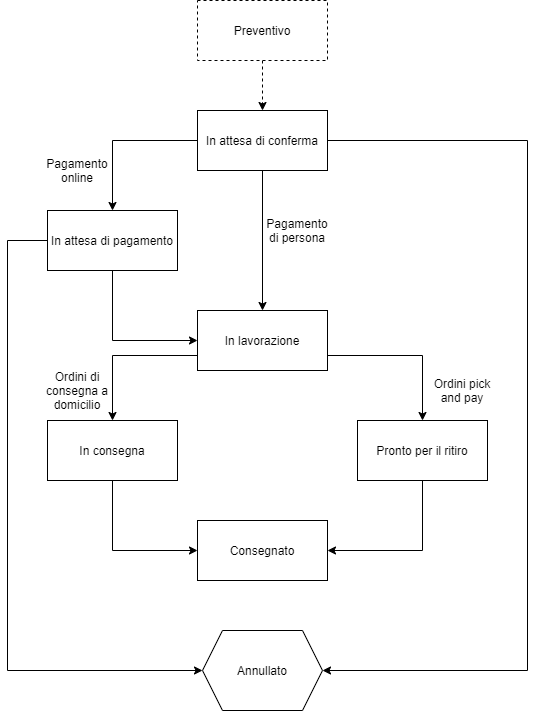
\includegraphics[width=1\linewidth]{statusord.png}
    \caption{Diagramma dei possibili stati di un ordine}
    \label{fig:subim2}
    \end{subfigure}
    
    \caption{Schermate di Garzone relative alle promozioni}
    \label{fig:image2}
\end{figure}
\FloatBarrier
\subsection{Preventivi}
Un ordine può essere anche generato da un negozio. Per eseguire questa operazione è necessario che il cliente richieda un preventivo al negozio. L'implementazione di questa funzionalità è stata prevista richiedendo ad un utente di inserire i dati necessari alla sua creazione, per poi generare un messaggio di chat che, invece di essere di tipo \textit{text}, è di tipo \textit{preventivo}. Il componente che effettua il render del messaggio di chat lato negozio interpreta automaticamente il messaggio di tipo preventivo e offre al negozio la possibilità di generare un preventivo tramite un modulo precompilato con i dati inseriti dall'utente. L'ordine sarà creato nello status \textit{preventivo} ed è questa volta compito dell'utente confermare o rifiutare il preventivo. In caso di divergenze tra domanda e offerta è possibile per il negozio modificare il preventivo creato e comunicarlo all'utente per poi consentire il preseguimento dell'evasione dell'ordine.
\section{Chat}
La Chat di Garzone permette di far comunicare tra loro un negozio ed un  cliente (One to One chat). L’idea alla base è quella di sfruttare in combinazione Firebase Realtime Database e Cloud SQL al fine di raggiungere il giusto compromesso tra performance, tempi di sviluppo e gestione dei costi. Firebase realtime Database si occuperà di salvare per ogni utente il counter delle notifiche e la sua lista di chat, mentre Cloud SQL salverà i messaggi (opzionalmente anche i contenitori chat). Firebase Realtime Database salverà per ogni utente, la lista delle sue chat oltre ai contatori di notifiche, in questo modo potrà essere sfruttata la funzionalità “real-time” per tenere aggiornata la lista chat e i badge di notifiche su tutti i client.\\
Secondo quanto sopracitato avremo un database che seguirà il qui descritto schema:
\begin{figure}[h!]
    \centering
    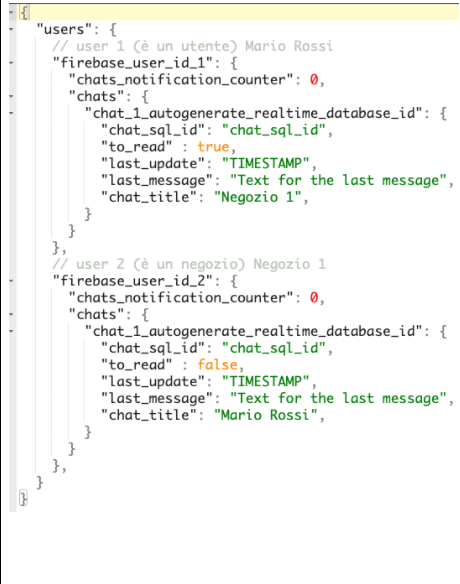
\includegraphics[width=0.5\textwidth]{chatrtd.png}
    \caption{Record di chat in Firebase Realtime Database}
\end{figure}
\FloatBarrier

\section{Appuntamenti}
Per la gestione appuntamenti è stato previsto l'utilizzo del package \lstinline[basicstyle=\ttfamily]!react-big-calendar! che offre un'interfaccia grafica ricca di funzionalità per creare e modificare eventi. Un utente può far uso dell'apposita funzionalità per richiedere un appuntamento ad un negozio. Viene quindi generato un messaggio di chat provvisto di richiesta, il quale viene automaticamente inviato al negozio. Sarà compito di quest'ultimo può creare l'appuntamento collegato al cliente che ne ha fatto richiesta. Nella pagina del negozio lato utente è possibile consultare gli slot orari disponibili, ovvero ancora non occupati dalla generazione di altri eventi, infatti in fase di creazione è previsto un filtraggio dei soli slot disponibili alla prenotazione.  
\begin{figure}[h!]
    \centering
    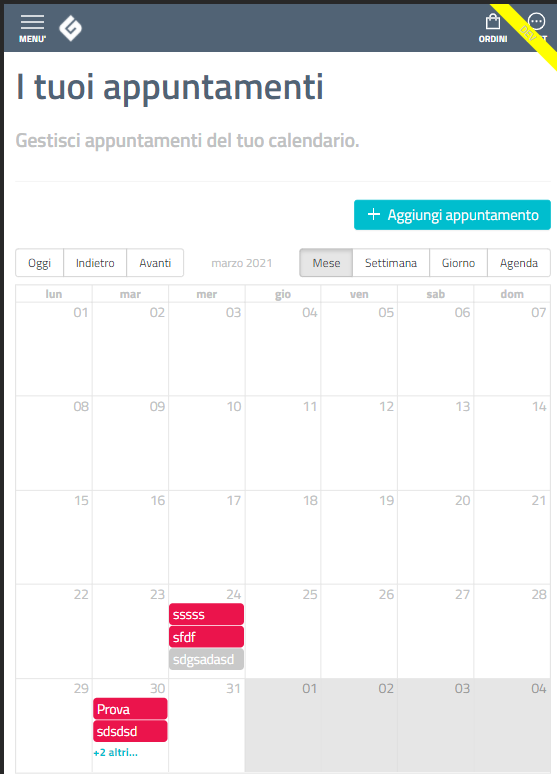
\includegraphics[width=0.8\textwidth]{app.png}
    \caption{Panoramica appuntamenti - Pannello negozio}
\end{figure}
\FloatBarrier